% DO NOT COMPILE THIS FILE DIRECTLY!
% This is included by the other .tex files.

\begin{frame}[t,plain]
\titlepage
\end{frame}

\begin{frame}{Structure of the talk}
	\tableofcontents
\end{frame}

\section{Tumor model}

\begin{frame}{Cahn-Hilliard equation}
	\begin{block}{}
		\vspace*{-0.2cm}
		\begin{equation*}
			\begin{aligned}
				u_t&= \nabla\cdot \left(M(u)\nabla\mu\right)\quad&\text{in }\Omega\times(0,T),\\
				\mu&=-\varepsilon^2\Delta u+F'(u)\quad&\text{in }\Omega\times(0,T),\\
				\nabla u\cdot \mathbf{n}&=M(u)\nabla\mu\cdot\mathbf{n}=0\quad&\text{on }\partial\Omega\times(0,T),\\
				u(0)&=u_0\quad&\text{in }\Omega.
			\end{aligned}
		\end{equation*}
	\end{block}
	\begin{itemize}
		\item $\alert{F(u)}=\frac{1}{4}u^2(1-u)^2$ Ginzburg-Landau double well functional.
		\item $\alert{M(u)}=u_\oplus(1-u)_\oplus$ degenerate mobility function.
		\begin{itemize}
			\item $v_\oplus \coloneqq\max\{v,0\}$,\quad
			$v_\ominus \coloneqq-\min\{v,0\},$\quad
			$v=v_\oplus  - v_\ominus$.
		\end{itemize}
		\item $u$ \structure{minimizes energy functional}:
		$$\alert{E(u(t))}\coloneqq\frac{\varepsilon^2}{2}\int_\Omega|\nabla u(t)|^2dx+\int_\Omega F(u(t))dx.$$
		\item Pointwise bounds: $u\in[0,1]$. 
	\end{itemize}
\end{frame}

\subsubsection{Tumor model}
\begin{frame}{Tumor model}
	\begin{block}{}
		\begin{center}
			\structure{\textbf{Cahn-Hilliard model (\alert{tumor})}} \alert{+} \structure{\textbf{Diffusion equation (\alert{nutrients})}}
		\end{center}
	\end{block}
	\begin{figure}[h!]
		\centering
		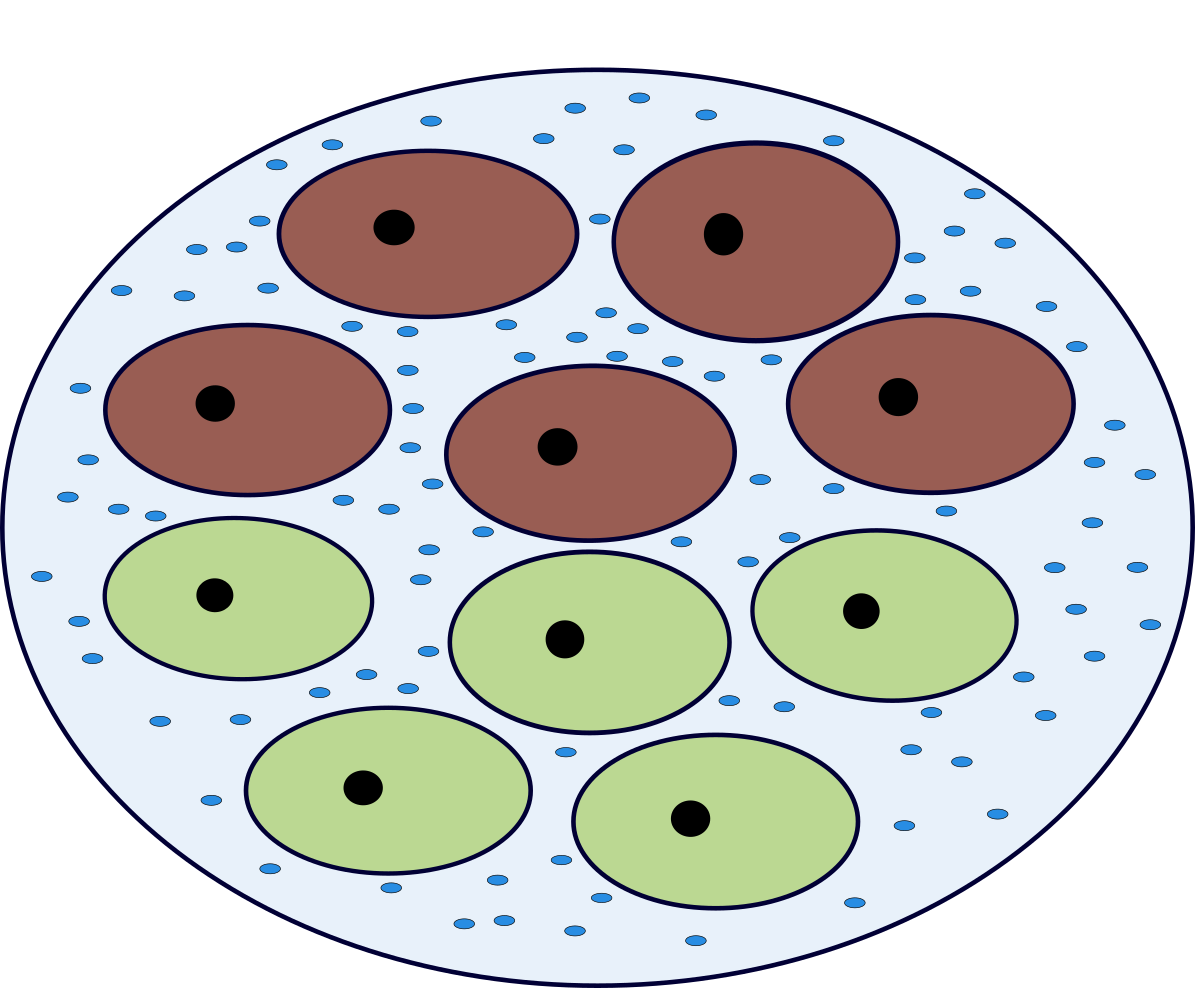
\includegraphics[scale=0.1]{img/celulas.png}
		\caption{Interaction between the species.}
	\end{figure}
	Variables $\alert{u}$ and $\alert{n}$ bounded on $[0,1]$:
	\begin{itemize}
		\item $\alert{u}$ phase-field variable ($1$ tumor cells and $0$ healthy cells).
		\item $\alert{n}$ nutrient-rich extracellular water volume fraction.
	\end{itemize}

	
	%	\structure{\textbf{energía}} $E\colon H^1(\Omega)\times H^1(\Omega)\longrightarrow\R$ se define como 
	%	\begin{align*}
		%	E(u(t),n(t))&\coloneqq\int_\Omega\left(\frac{\varepsilon^2}{2}|\nabla u(x,t)|^2+F(u(x,t))-\chi_0u(x,t)n(x,t)+\frac{1}{2\delta}\left(n(x,t)\right)^2\right)dx.
		%	\end{align*}
\end{frame}

\begin{frame}{Tumor model {\footnotesize (derived from \cite{van_der_zee_model})}}
	\footnotesize
	\vspace*{-0.2cm}
	\begin{block}{}
		\vspace*{-0.4cm}
		\begin{subequations}
			\begin{align*}
				\partial_t u&=C_u\nabla\cdot\left(M(u)\nabla\mu_u\right)+\framedmath<2>{\delta P_0P(u,n)(\mu_n-\mu_u)_\oplus} \quad&\text{in }\Omega\times (0,T),\\
				\mu_u&=F'(u)-\varepsilon^2\Delta u\framedmath<3>{-\chi_0 n}\quad&\text{in }\Omega\times (0,T),\\
				\partial_t n&=C_n\nabla\cdot\left(M(n)\nabla\mu_n\right)-\framedmath<2>{\delta P_0P(u,n)(\mu_n-\mu_u)_\oplus} \quad&\text{in }\Omega\times (0,T),\\
				\mu_n&=\frac{1}{\delta} n \framedmath<3>{-\chi_0 u} \quad&\text{in }\Omega\times (0,T),\\
				\nabla u\cdot \mathbf{n}&=\left( M(n)\nabla \mu_n\right)\cdot \mathbf{n}=\left( M(u)\nabla \mu_u\right)\cdot \mathbf{n}=0 \quad &\text{on }\partial\Omega\times (0,T),\\
				u(0)&=u_0,\quad n(0)=n_0\quad&\text{in }\Omega,%\\
				%\mu_u(0)&=f'(u_0)-\varepsilon^2\Delta u_0-\chi_0 n_0\quad&\text{en }\Omega,
			\end{align*}
		\end{subequations}
	\end{block}
	where $u_0,n_0\in L^2(\Omega)$are the initial conditions.
	
	\vspace*{0.2cm}
	\begin{itemize}
		\item $\alert{M(v)}\coloneqq h_{p,q}(v)$, $\alert{P(u,n)}\coloneqq h_{r,s}(u)n_\oplus$ for certain $p,q,r,s\in\N$, where 
		$$
		\alert{h_{p,q}(v)}\coloneqq K_{p,q}v_\oplus^p(1-v)_\oplus^q
		$$
		with $K_{p,q}>0$ a constant so that $\max_{x\in\R}h_{p,q}(v)=1$.
		\item<2> \myframed{Cells-nutrients chemical reactions.}
		\item<3> \myframed{Movement of tumor cells $\longleftarrow$ \textbf{Cross-diffusion terms}.}
	\end{itemize}	
\end{frame}

\begin{frame}{Properties of the model}
	\begin{proposition}[Mass conservation]
		The total mass of tumor cells and nutrients is conserved: $$\alert{\frac{d}{dt}\int_\Omega (u(x,t)+n(x,t))dx=0}.$$
	\end{proposition}
	\begin{proposition}[Pointwise bounds]
		Let $u_0,v_0\in[0,1]$, then \alert{$u(t),n(t)\in[0,1]$} for a.e. $t\in(0,T)$.
	\end{proposition}
	\vspace*{0.6cm}
\end{frame}
\begin{frame}{Properties of the model}
	\scriptsize
	\begin{proposition}[Energy law]
		If $\partial_t u\in L^2(0,T, H^1(\Omega))$, then it satisfies the following energy law
		\begin{align*}
			\frac{d E(u(t),n(t))}{dt}&+C_u\int_\Omega M(u(x,t))|\nabla\mu_u(x,t)|^2dx+C_n\int_\Omega M(n(x,t))|\nabla\mu_n(x,t)|^2\notag\\&+\delta P_0\int_\Omega P(u(x,t),n(x,t))(\mu_u(x,t)-\mu_n(x,t))_\oplus ^2dx=0,
		\end{align*}
		where
		\begin{align*}
			\alert{E(u(t),n(t))}&\coloneqq\int_\Omega\left(\frac{\varepsilon^2}{2}|\nabla u(x,t)|^2+ F(u(x,t))-\chi_0u(x,t)n(x,t)+\frac{1}{2\delta}\left(n(x,t)\right)^2\right)dx.
		\end{align*}
		Therefore, the solution is \structure{energy stable} in the sense $$\alert{\frac{d}{dt}E(u(t),n(t))\le 0}.$$
	\end{proposition}
\end{frame}

\section{Approximation of the model}
\begin{frame}{FE and DG methods}
	\footnotesize
	\vspace*{-0.2cm}
	\begin{block}{}
		\text{Finite Element method:}
		\begin{equation*}
			\alert{\Pc_k(\T_h)}\coloneqq\left\{v_h\in \mathcal{C}^0(\overline\Omega)\colon v_{h|_{K_i}}\in\mathbb{P}_k(K_i)\text{ with } K_i\in\T_h,\forall i\in\left\{1,2,\ldots,N_{\T_h}\right\}\right\},
		\end{equation*}
		\text{Discontinuous Galerkin method:}
		\begin{equation*}
			\alert{\Pd_k(\T_h)}\coloneqq\left\{v_h\in L^2(\Omega)\colon v_{h|_{K_i}}\in\mathbb{P}_k(K_i)\text{ with } K_i\in\T_h,\forall i\in\left\{1,2,\ldots,N_{\T_h}\right\}\right\}.
		\end{equation*}
	\end{block}
	% with a basis $\left\{\phi_i\right\}_{i\in\left\{1,2,\ldots,N_h \right\}}$.
	
	\vspace*{0.3cm}
	Notation:
	
	\begin{minipage}{0.69\textwidth}
	\begin{itemize}
		\item \structure{Average}: 
		$\alert{\media{v}}\coloneqq
		\begin{cases}
			\dfrac{\vK+\vL}{2}&\text{if } e=\partial K\cap\partial L\in\E_h^i\\
			\vK&\text{if }e=\partial K\in\E_h^b
		\end{cases},$
		\item \structure{Jump}: $
		\alert{\salto{v}}\coloneqq
		\begin{cases}
			\vK-\vL&\text{if } e=\partial K\cap\partial L\in\E_h^i\\
			\vK&\text{if }e=\partial K\in\E_h^b
		\end{cases},$
	\end{itemize}
	\end{minipage}
	\begin{minipage}{0.29\textwidth}
		\vspace*{-0.5cm}
		\begin{figure}
			\centering
			\includegraphics[scale=0.7]{img/orientation_n.pdf}
			{\scriptsize\structure{Figure:} Orientation of unit normal vector.}
		\end{figure}
	\end{minipage}
\end{frame}

\begin{frame}{Projection and regularization operators}
	Let $g\in L^1(\Omega)$.
	\vspace*{0.3cm}

	\begin{itemize}
		\item \structure{Projection} $\alert{\Pi_0}\colon L^1(\Omega) \rightarrow \Pd_0(\T_h)$:
		\begin{equation*}
			\escalarL{g}{\overline{w}}=
			\escalarL{\alert{\Pi_0 g}}{\overline{w}},\forall\,\overline{w}\in \Pd_0(\T_h).
		\end{equation*}
		\vspace*{0.1cm}
		\item \structure{Regularization} $\alert{\Pi^h_1}\colon L^1(\Omega)\rightarrow \Pc_1(\T_h)$
		\begin{equation*}
			\escalarL{g}{\overline{\phi}}=\escalarML{\alert{\Pi^h_1 g}}{\overline{\phi}},\forall\,\overline{\phi}\in \Pc_1(\T_h),
		\end{equation*}
		where $\alert{\escalarML{\cdot}{\cdot}}$ is the \structure{mass-lumping scalar product} in $\Pc_1(\T_h)$.
	\end{itemize}
\end{frame}

\begin{frame}{Mesh assumptions}
	\begin{hypothesis}
		\label{hyp:mesh_n}
		The mesh $\T_h$ of $\overline\Omega$ is structured in the sense that the line between the baricenters of the triangles $K$ and $L$ is orthogonal to the interface $e=K\cap L\in\E_h^i$.
	\end{hypothesis}
	\vspace*{0.5cm}
	\begin{figure}
		\centering
		\includegraphics[scale=0.55]{img/adjacent_baricenters.pdf}
		\caption{Polygonal structure between adjacent baricenters.}
	\end{figure}
\end{frame}
\begin{frame}{Mesh assumptions}
	With this assumption:
	$$\nabla\mu \cdot \nn_e \simeq\frac{-\salto{\Pi_0\mu}}{\mathcal{D}_e(\T_h)}= \frac{\Pi_0\mu_L-\Pi_0\mu_K}{\mathcal{D}_e(\T_h)}\eqqcolon \alert{\nabla_{\nn_e}^0\mu},$$
	on every $e=K\cap L\in\Ehi$ with $\alert{\mathcal{D}_e(\T_h)}$ the distance between the baricenters of the triangles $K$ and $L$.

	\vspace*{0.3cm}
	\begin{block}{}
		For $\mu\in\Pd_1(\T_h)$, $\nabla_{\nn_e}^0\mu$ is the slope of the line between $(C_K, \mu(C_K))$ and $(C_L, \mu(C_L))$, with $C_K, C_L$ the baricenters of $K, L\in\T_h$.
	\end{block}
	\vspace*{0.3cm}
	More information in \cite{acosta-soba_KS_2022}.
\end{frame}

\begin{frame}{Upwind method {\footnotesize (derived from \cite{acosta-soba_CH_2022})}}
	\footnotesize
	Notice that
	$$\nabla\cdot(M(v)\nabla\mu)=M'(v)\nabla\mu \cdot\nabla v+M(v)\Delta\mu.$$
	Hence, $\alert{M'(v)}$ determines the direction of the flux.
	
	\vspace*{0.3cm}
	% \begin{itemize}
	% 	\item If $u\in[0,1]$ then $M(u)=M(u)_\oplus$.
	% \end{itemize}
	% \vspace*{0.3cm}
	
	Consider $M(v)=M^\uparrow(v)+M^\downarrow(v)$:
	\begin{itemize}
		\item Increasing part of $M(v)$: $\alert{M^\uparrow(v)}=
		\begin{cases}
			M(v) & \text{if }v\le \frac{1}{2}\\[0.2em]
			M\left(\frac{1}{2}\right) & \text{if } v>\frac{1}{2}
		\end{cases}.$
		\item Decreasing part of $M(v)$: $
		\alert{M^\downarrow(v)}=
		\begin{cases}
			0 & \text{if }v\le \frac{1}{2}\\
			M(v)-M\left(\frac{1}{2}\right) & \text{if } v>\frac{1}{2}
		\end{cases}.$
	\end{itemize}

	% \vspace*{0.3cm}
	\begin{block}{}
	$a_h^{\text{upw}}:\Pd_k(\T_h)\times \Pd_k(\T_h)\to\R$,
	\scriptsize
	\begin{multline*}
		\alert{\aupw{\mu}{M(v)}{\bv}}\coloneqq-\int_\Omega (\nabla\mu\cdot\nabla\overline{v})M(v)\\+\sum_{e\in\E_h^i,e=K\cap L}\int_e\left((\nabla_{\nn_e}^0\mu)_{\oplus}(M^\uparrow(\vK)+M^\downarrow(\vL))_\oplus-(\nabla_{\nn_e}^0\mu)_{\ominus}(M^\uparrow(\vL)+M^\downarrow(\vK))_\oplus\right)\salto{\bv}
	\end{multline*}
	\end{block}
\end{frame}

\begin{frame}{Numerical scheme}
	\footnotesize
	Given $u^m,n^m\in\Pd_0(\T_h)$ with $u^{m},n^{m}\in[0,1]$ and $\mu_u^m\in\Pc_1(\T_h)$, find $u^{m+1}, n^{m+1}\in \Pd_0(\T_h)$ and $\mu_u^{m+1} \in \Pc_1(\T_h)$, such that
	\begin{block}{}
		\begin{align*}
			\escalarL{\delta_tu^{m+1}}{\overline{u}}&=-C_u\aupw{\mu_u^{m+1}}{M(u^{m+1})}{\overline{u}}&\notag\\&\quad+\delta P_0\escalarL{P(u^{m+1},n^{m+1})(\mu_n^{m+1}-\Pi_0\mu_u^{m+1})_\oplus }{\overline{u}},\\
			\escalarML{\mu_u^{m+1}}{\overline{\mu}_u}&=\varepsilon^2 \escalarLd{\nabla \up^{m+1}}{\nabla\overline{\mu}_u}+ \escalarL{f(\up^{m+1},\up^m)}{\overline{\mu}_u}\nonumber\\&\quad-\chi_0\escalarL{ n^{m+1}}{\overline{\mu}_u},\\
			\escalarL{\delta_t n^{m+1}}{\overline{n}}&=-C_n\aupw{\mu_n^{m+1}}{M(n^{m+1})}{\overline{n}}&\notag\\&\quad-\delta P_0 \escalarL{P(u^{m+1},n^{m+1})(\mu_n^{m+1}-\Pi_0\mu_u^{m+1})_\oplus }{\overline{n}},\\
			\mu_n^{m+1}&=\frac{1}{\delta}n^{m+1}  -\chi_0 \Pi_0(\up^{m}),
		\end{align*}
	\end{block}
	$\forall\overline{u},\overline{n}\in\Pd_0(\T_h)$, $\forall\overline{\mu}_u\in \Pc_1(\T_h)$, where $u^0=u_0$, $n^0=n_0$
\end{frame}

\begin{frame}{Properties of the discrete scheme}
	\begin{proposition}[Mass conservation]
		The total mass of cells and nutrients is conserved: for all $m\ge 0$,
		\footnotesize
		\begin{align*}
		\alert{\int_\Omega (u^{m+1}+n^{m+1})=\int_\Omega (u^m+n^m)}\quad\text{and}\quad\alert{\int_\Omega (\up^{m+1}+n^{m+1})=\int_\Omega (\up^m+n^m)}.
		\end{align*}
	\end{proposition}
	\vspace*{0.3cm}
	\begin{theorem}[Pointwise bounds]
		Let $u^{m},n^{m}\in[0,1]$, then $\alert{u^{m+1},\up^{m+1},n^{m+1}\in[0,1]}$.
	\end{theorem}
	\vspace*{0.3cm}
	\begin{theorem}[Existence of solution]
		There is at least one solution of the scheme.
	\end{theorem}
\end{frame}
\begin{frame}{Properties of the discrete scheme}
	\begin{theorem}[Energy law]
		Any solution satisfies the following discrete energy law
		{\footnotesize
		\begin{align*}
			\delta_t E(\up^{m+1},n^{m+1})&+C_u\aupw{\mup_u^{m+1}}{M(u^{m+1})}{\Pi_0\mu_u^{m+1}}\\&+C_n\aupw{\mu_n^{m+1}}{M(n^{m+1})}{\mu_n^{m+1}}\notag\\&+\frac{\Delta t\varepsilon^2}{2}\int_\Omega|\delta_t\nabla \up^{m+1}|^2+\frac{\Delta t}{2\delta}\int_\Omega \vert\delta_t n^{m+1}\vert^2\nonumber\\&+\delta P_0\int_\Omega P(u^{m+1},n^{m+1}) (\mu_n^{m+1}-\mup_u^{m+1})_\oplus ^2
			\le 0.
		\end{align*}
		}
	\end{theorem}
	\begin{corollary}[Energy stability]
		The scheme is \structure{unconditionally energy stable} in the sense
		$$
		\alert{E(\up^{m+1},n^{m+1})\le E(\up^{m},n^{m})}.
		$$
	\end{corollary}
\end{frame}

\section{Numerical tests}

\subsection{Three tumors aggregation}

\begin{frame}{Three tumors aggregation}
	% {\tiny
	% \begin{align*}
	% 	u_0 &= \frac{1}{2}\left[\tanh\left(\frac{1 - \sqrt{(x- 2)^2 + (y - 2)^2}}{\sqrt{2}\varepsilon}\right)
	% 	+ \tanh\left(\frac{1 - \sqrt{(x - 3)^2 + (y + 5)^2}}{\sqrt{2}\varepsilon}\right)\right.\\&\quad\left.
	% 	+ \tanh\left(\frac{1.73 - \sqrt{(x + 1.5)^2 + (y + 1.5)^2}}{\sqrt{2}\varepsilon}\right) + 3\right],\\
	% 	n_0 &= 1.0 - u_0.
	% \end{align*}}

	\begin{figure}
		\centering
		\begin{tabular}{cc}
			\hspace*{-0.9cm}$\boldsymbol{u_0}$ & \hspace*{-0.9cm}$\boldsymbol{n_0}$\\
			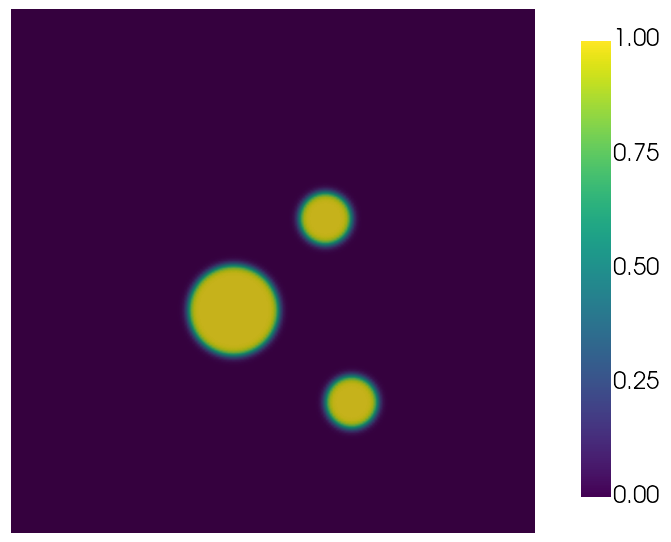
\includegraphics[scale=0.2]{img/three_tumors/initial_cond/tumor_DG-UPW_Pi1_u_i-0_cropped.png} &
			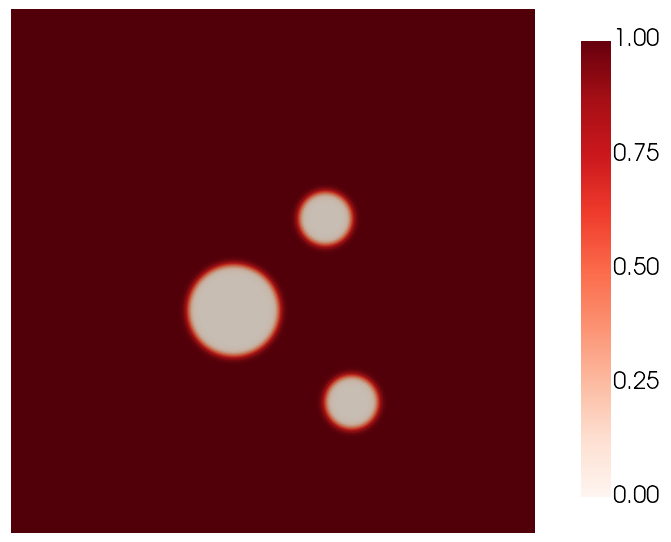
\includegraphics[scale=0.2]{img/three_tumors/initial_cond/tumor_DG-UPW_Pi1_n_i-0_cropped.png}
		\end{tabular}
		% \caption{Initial conditions for test \ref{sec:numer-experiments_1} ($u_0$ left, $n_0$ right).}
	\end{figure}

	Symmetric mobility and proliferation functions:
	$$
	M(v)=h_{1,1}(v),\quad P(u,n)=h_{1,1}(u)n_\oplus.
	$$

	Parameters: $C_u=100$, $C_n=100\cdot 10^{-4}$, $P_0=125$,  $h\approx 0.14$.
\end{frame}

\begin{frame}{Three tumors aggregation ($\chi_0=0$, $\Delta t=10^{-5}$)}
	\scriptsize
	\begin{figure}
		\centering
		\hspace*{-0.6cm}
		\begin{tabular}{cccc}
			&\hspace*{-1cm}$t=2.5\cdot 10^{-2}$ & \hspace*{-1cm}$t=5.0\cdot 10^{-2}$ & \hspace*{-1cm}$t=7.5\cdot 10^{-2}$ \\
			\rotatebox[origin=c]{90}{\textbf{DG}} &
			\raisebox{-0.47\height}{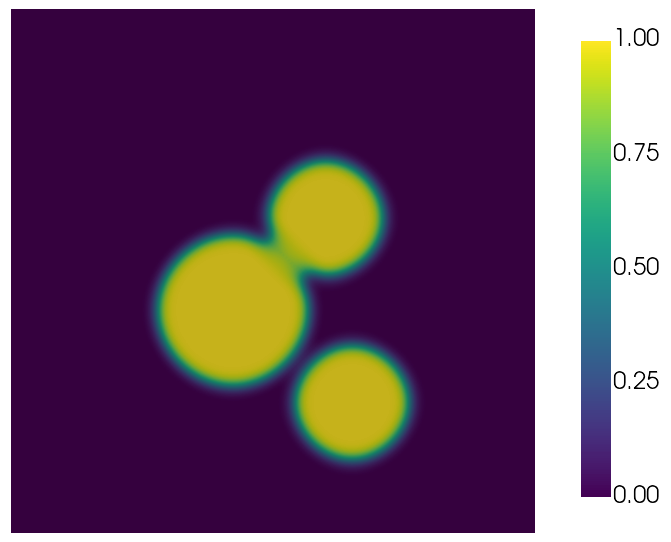
\includegraphics[scale=0.145]{img/three_tumors/test_DG_P0-125_dt-1e-5_nx-200_symmetric/tumor_DG-UPW_Pi1_u_i-2500_cropped.png}} &
			\raisebox{-0.47\height}{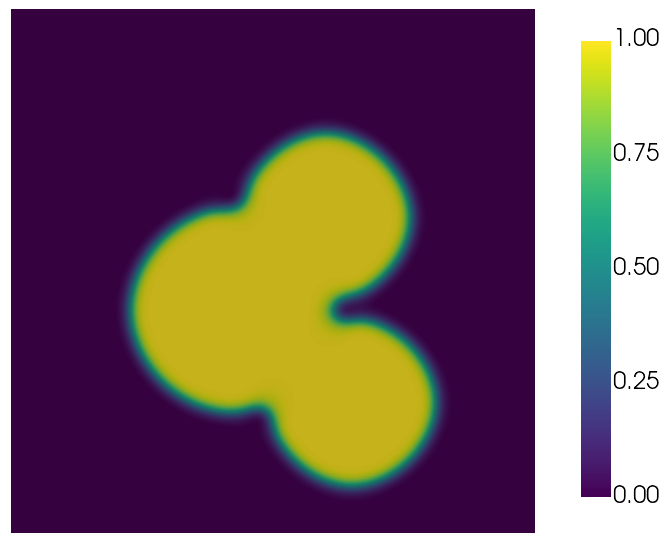
\includegraphics[scale=0.145]{img/three_tumors/test_DG_P0-125_dt-1e-5_nx-200_symmetric/tumor_DG-UPW_Pi1_u_i-5000_cropped.png}} &
			\raisebox{-0.47\height}{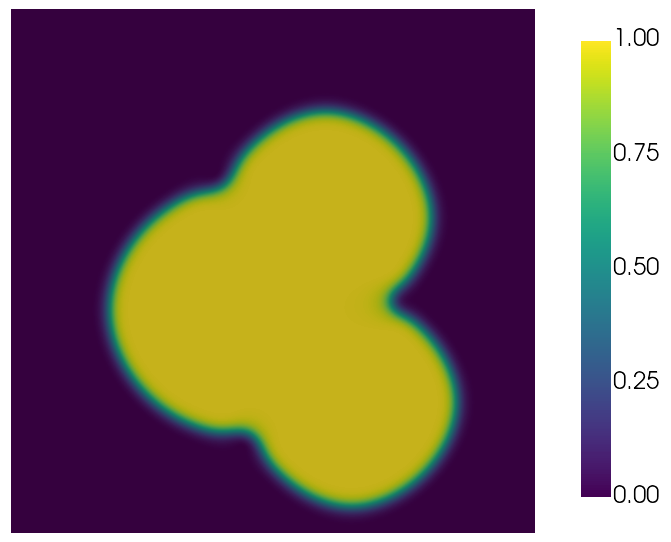
\includegraphics[scale=0.145]{img/three_tumors/test_DG_P0-125_dt-1e-5_nx-200_symmetric/tumor_DG-UPW_Pi1_u_i-7500_cropped.png}} \\
			\rotatebox[origin=c]{90}{\textbf{FE}} &
			\raisebox{-0.47\height}{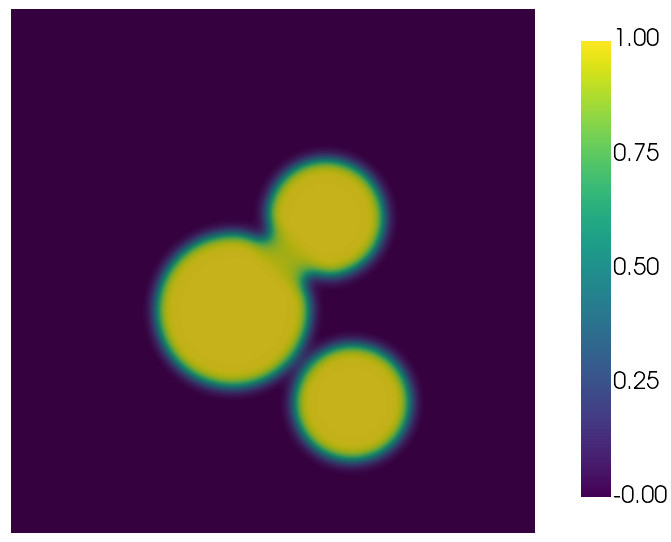
\includegraphics[scale=0.145]{img/three_tumors/test_FEM_P0-125_dt-1e-5_nx-200_symmetric/tumor_FEM_u_i-2500_cropped.png}} &
			\raisebox{-0.47\height}{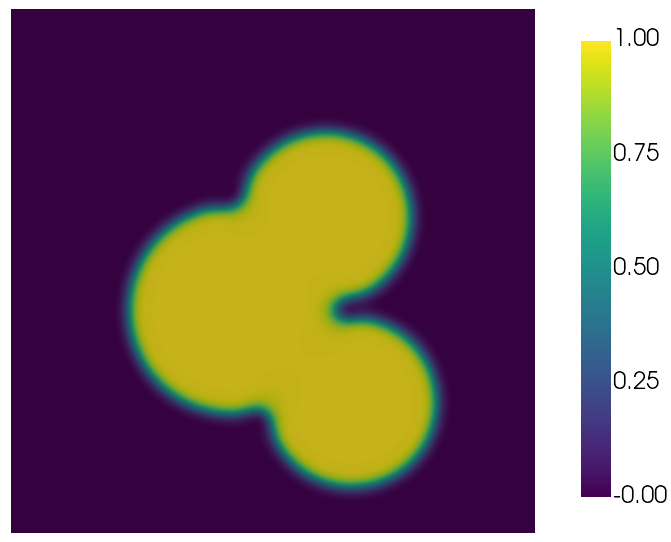
\includegraphics[scale=0.145]{img/three_tumors/test_FEM_P0-125_dt-1e-5_nx-200_symmetric/tumor_FEM_u_i-5000_cropped.png}} &
			\raisebox{-0.47\height}{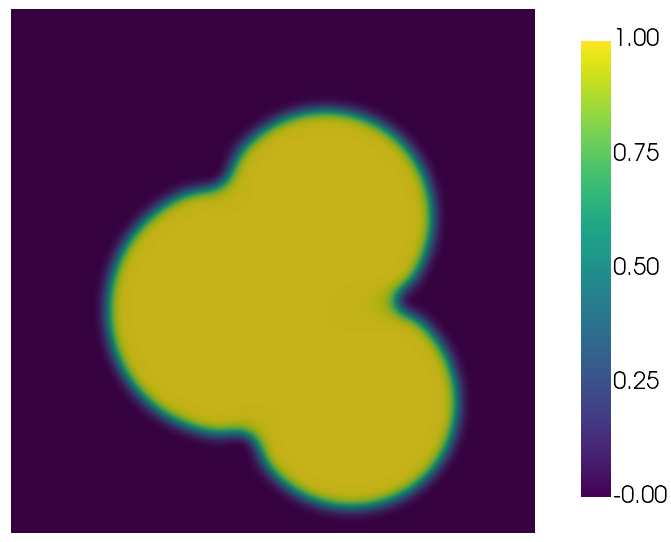
\includegraphics[scale=0.145]{img/three_tumors/test_FEM_P0-125_dt-1e-5_nx-200_symmetric/tumor_FEM_u_i-7500_cropped.png}}
		\end{tabular}
		\caption{Tumor cells.}
	\end{figure}
\end{frame}
\begin{frame}{Three tumors aggregation ($\chi_0=0$, $\Delta t=10^{-5}$)}
	\scriptsize
	\begin{figure}
		\centering
		\hspace*{-0.6cm}
		\begin{tabular}{cccc}
			&\hspace*{-1cm}$t=2.5\cdot 10^{-2}$ & \hspace*{-1cm}$t=5.0\cdot 10^{-2}$ & \hspace*{-1cm}$t=7.5\cdot 10^{-2}$ \\
			\rotatebox[origin=c]{90}{\textbf{DG}} &
			\raisebox{-0.47\height}{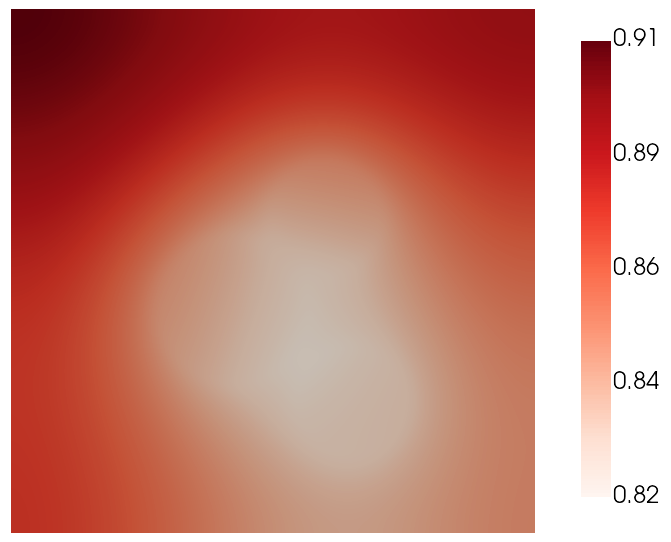
\includegraphics[scale=0.145]{img/three_tumors/test_DG_P0-125_dt-1e-5_nx-200_symmetric/tumor_DG-UPW_Pi1_n_i-2500_cropped.png}} &
			\raisebox{-0.47\height}{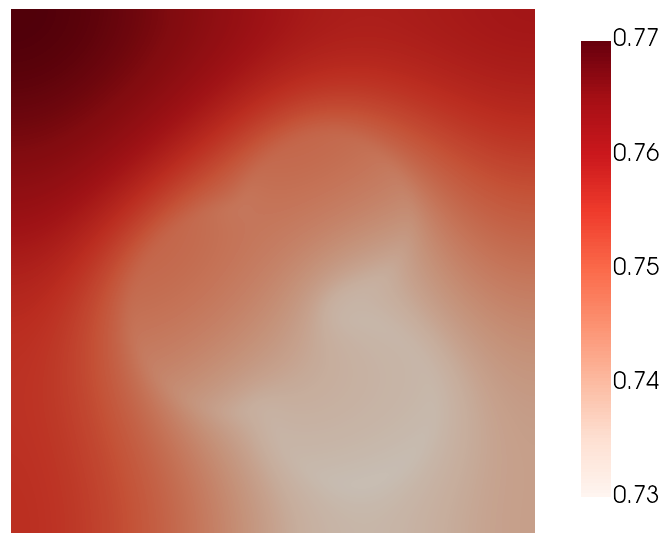
\includegraphics[scale=0.145]{img/three_tumors/test_DG_P0-125_dt-1e-5_nx-200_symmetric/tumor_DG-UPW_Pi1_n_i-5000_cropped.png}} &
			\raisebox{-0.47\height}{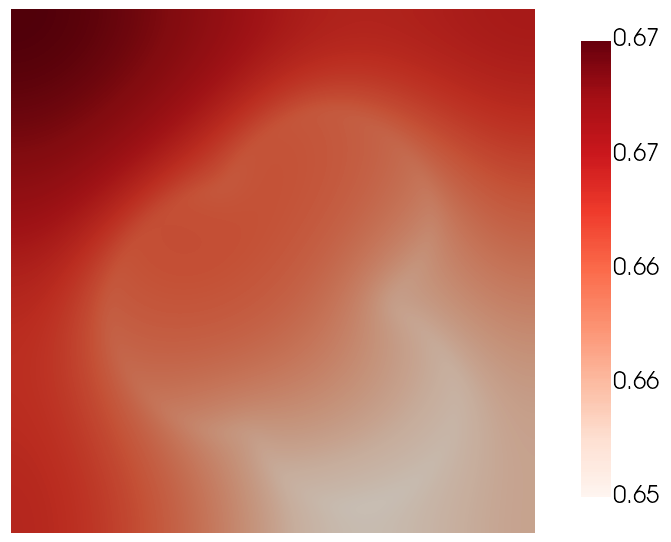
\includegraphics[scale=0.145]{img/three_tumors/test_DG_P0-125_dt-1e-5_nx-200_symmetric/tumor_DG-UPW_Pi1_n_i-7500_cropped.png}} \\
			\rotatebox[origin=c]{90}{\textbf{FE}} &
			\raisebox{-0.47\height}{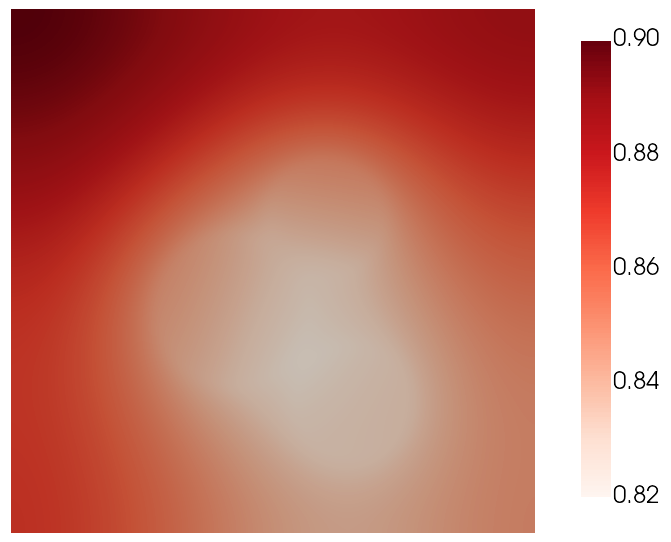
\includegraphics[scale=0.145]{img/three_tumors/test_FEM_P0-125_dt-1e-5_nx-200_symmetric/tumor_FEM_n_i-2500_cropped.png}} &
			\raisebox{-0.47\height}{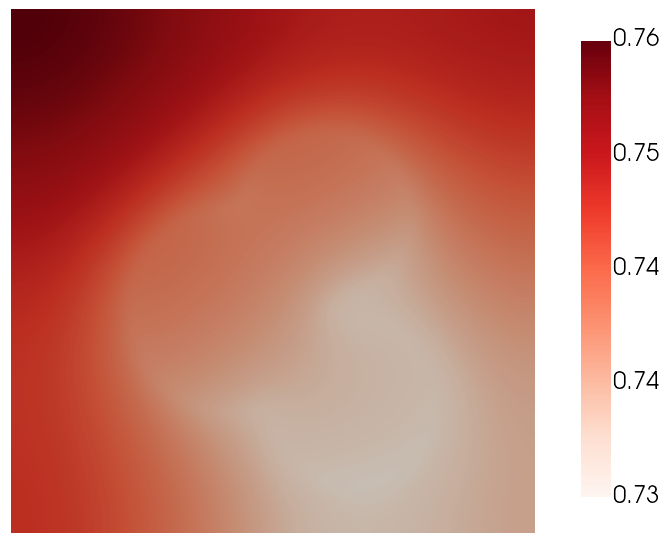
\includegraphics[scale=0.145]{img/three_tumors/test_FEM_P0-125_dt-1e-5_nx-200_symmetric/tumor_FEM_n_i-5000_cropped.png}} &
			\raisebox{-0.47\height}{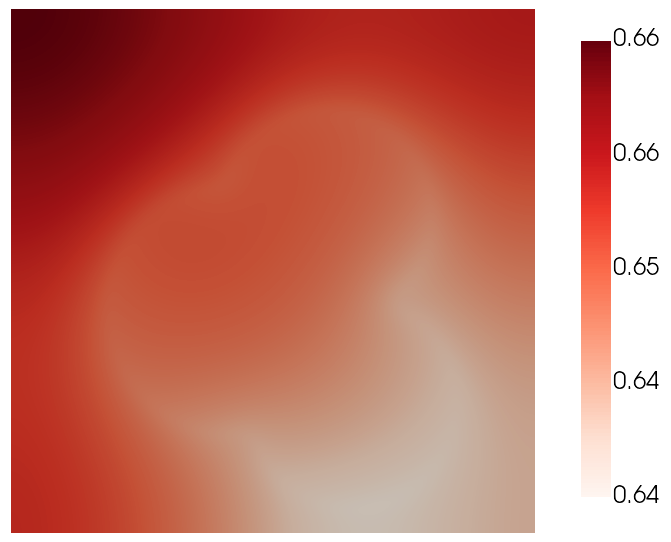
\includegraphics[scale=0.145]{img/three_tumors/test_FEM_P0-125_dt-1e-5_nx-200_symmetric/tumor_FEM_n_i-7500_cropped.png}}
		\end{tabular}
		\caption{Nutrients.}
		% \label{fig:test-1_1}
	\end{figure}
\end{frame}
\begin{frame}{Three tumors aggregation ($\chi_0=0$, $\Delta t=10^{-5}$)}
	\begin{figure}
		\centering
		\begin{tabular}{cc}
			\hspace*{1cm}$\boldsymbol{u}$ & \hspace*{0.5cm}$\boldsymbol{n}$\\
			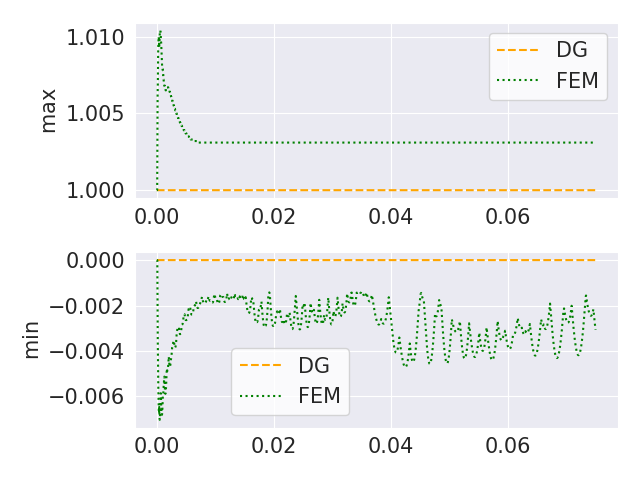
\includegraphics[scale=0.33]{img/three_tumors/tumor_min-max_u_chi-0.png} &
			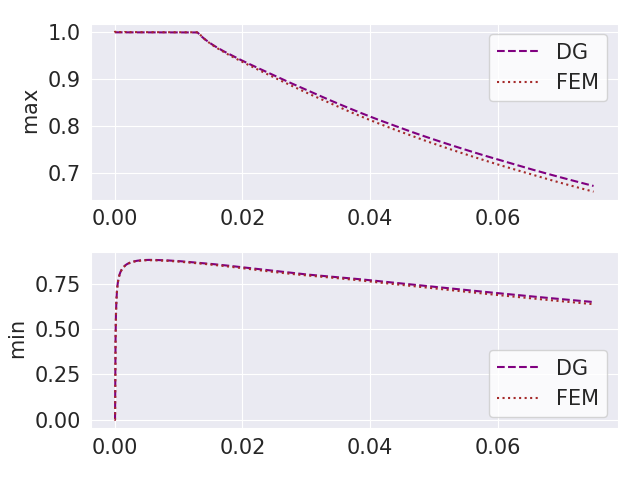
\includegraphics[scale=0.33]{img/three_tumors/tumor_min-max_n_chi-0.png}
		\end{tabular}
		\caption{Pointwise bounds.}
	\end{figure}
\end{frame}
\begin{frame}{Three tumors aggregation ($\chi_0=0$, $\Delta t=10^{-5}$)}
	\begin{figure}
		\centering
		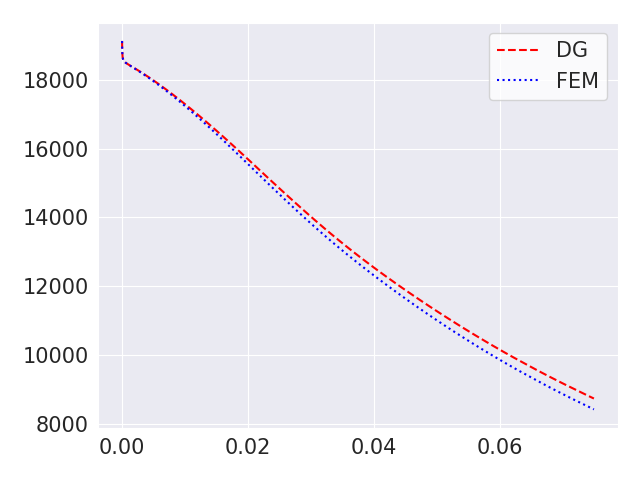
\includegraphics[scale=0.45]{img/three_tumors/tumor_energy_chi-0.png}
		\caption{Energy.}
	\end{figure}
\end{frame}

\begin{frame}{Three tumors aggregation ($\chi_0=10$, $\Delta t=6\cdot 10^{-5}$)}
	\scriptsize
	\begin{figure}
		\centering
		\hspace*{-0.6cm}
		\begin{tabular}{cccc}
			& \hspace*{-1cm}$t=7.5\cdot 10^{-3}$ & \hspace*{-1cm}$t=1.5\cdot 10^{-2}$ & \hspace*{-1cm}$t=4\cdot 10^{-2}$ \\
			\rotatebox[origin=c]{90}{\textbf{DG}} &
			\raisebox{-0.47\height}{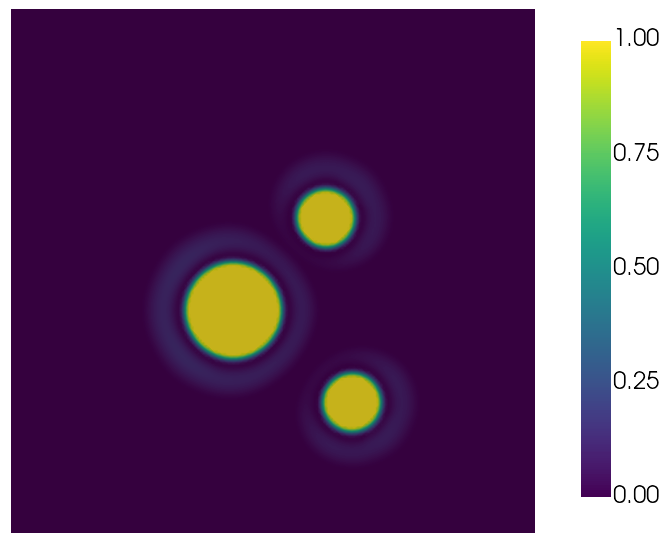
\includegraphics[scale=0.145]{img/three_tumors/test_DG_P0-125_chi-10_dt-5e-6_nx-200_symmetric/tumor_DG-UPW_Pi1_u_i-1500_cropped.png}} &
			\raisebox{-0.47\height}{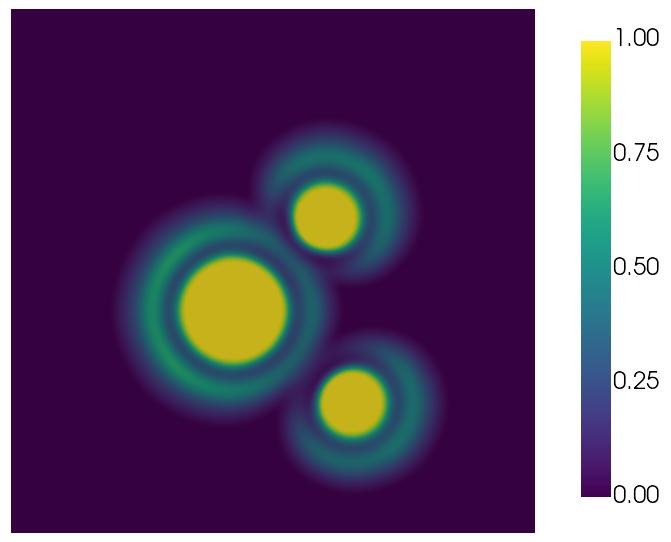
\includegraphics[scale=0.145]{img/three_tumors/test_DG_P0-125_chi-10_dt-5e-6_nx-200_symmetric/tumor_DG-UPW_Pi1_u_i-3000_cropped.png}} &
			\raisebox{-0.47\height}{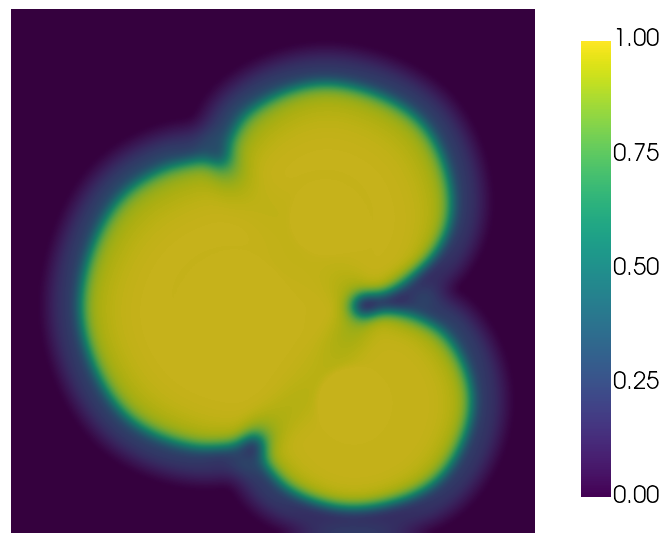
\includegraphics[scale=0.145]{img/three_tumors/test_DG_P0-125_chi-10_dt-5e-6_nx-200_symmetric/tumor_DG-UPW_Pi1_u_i-8000_cropped.png}} \\
			\rotatebox[origin=c]{90}{\textbf{FE}} &
			\raisebox{-0.47\height}{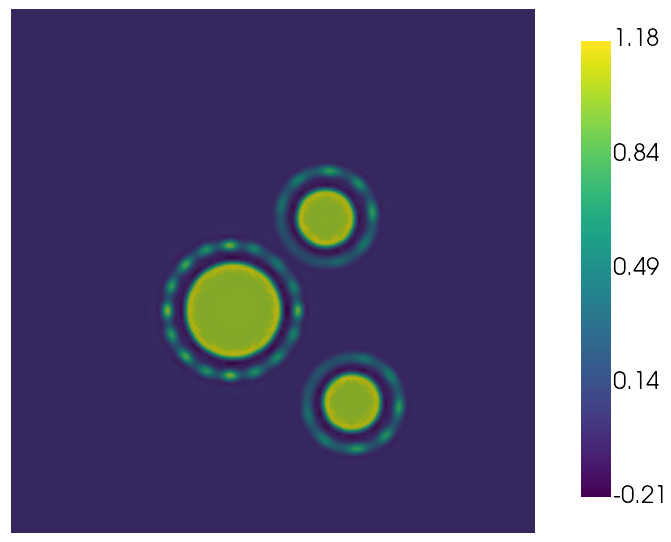
\includegraphics[scale=0.145]{img/three_tumors/test_FEM_P0-125_chi-10_dt-5e-6_nx-200_symmetric/tumor_FEM_u_i-1500_cropped.png}} &
			\raisebox{-0.47\height}{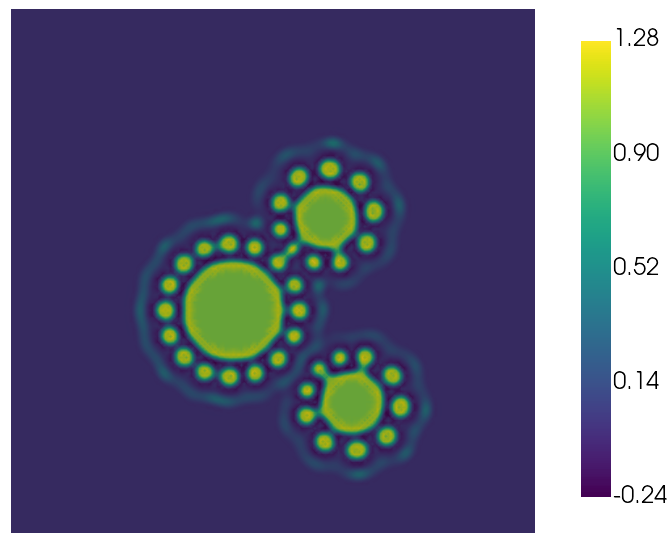
\includegraphics[scale=0.145]{img/three_tumors/test_FEM_P0-125_chi-10_dt-5e-6_nx-200_symmetric/tumor_FEM_u_i-3000_cropped.png}} &
			\raisebox{-0.47\height}{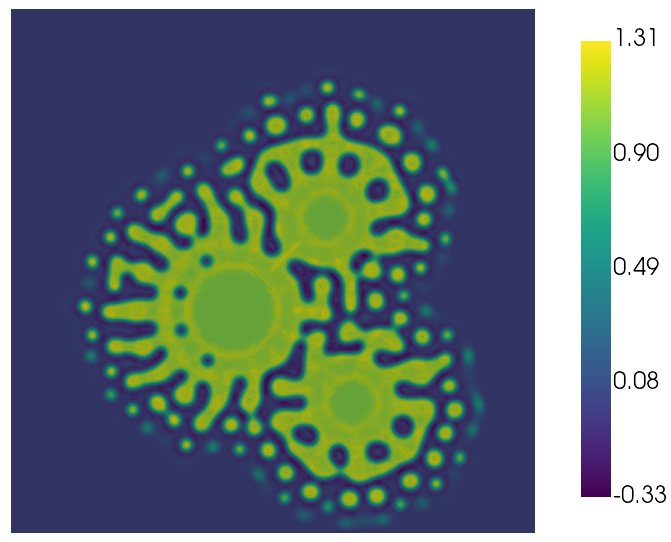
\includegraphics[scale=0.145]{img/three_tumors/test_FEM_P0-125_chi-10_dt-5e-6_nx-200_symmetric/tumor_FEM_u_i-8000_cropped.png}}
		\end{tabular}
		\caption{Tumor cells.}
	\end{figure}
\end{frame}
\begin{frame}{Three tumors aggregation ($\chi_0=10$, $\Delta t=6\cdot 10^{-5}$)}
	\scriptsize
	\begin{figure}
		\centering
		\hspace*{-0.6cm}
		\begin{tabular}{cccc}
			& \hspace*{-1cm}$t=7.5\cdot 10^{-3}$ & \hspace*{-1cm}$t=1.5\cdot 10^{-2}$ & \hspace*{-1cm}$t=4\cdot 10^{-2}$ \\
			\rotatebox[origin=c]{90}{\textbf{DG}} &
			\raisebox{-0.47\height}{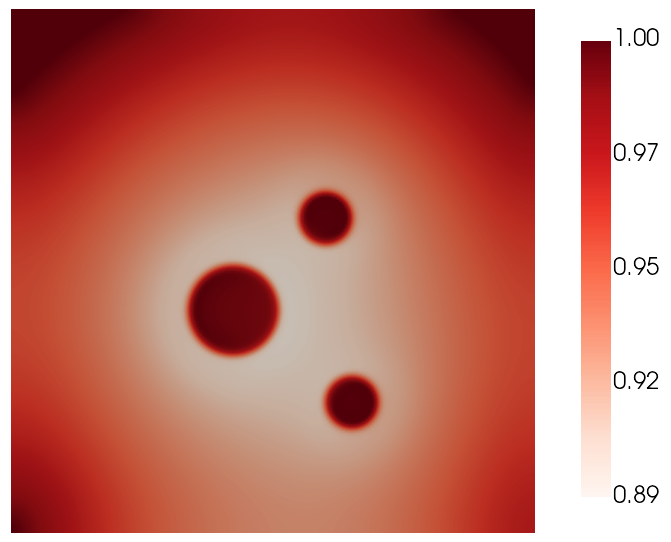
\includegraphics[scale=0.145]{img/three_tumors/test_DG_P0-125_chi-10_dt-5e-6_nx-200_symmetric/tumor_DG-UPW_Pi1_n_i-1500_cropped.png}} &
			\raisebox{-0.47\height}{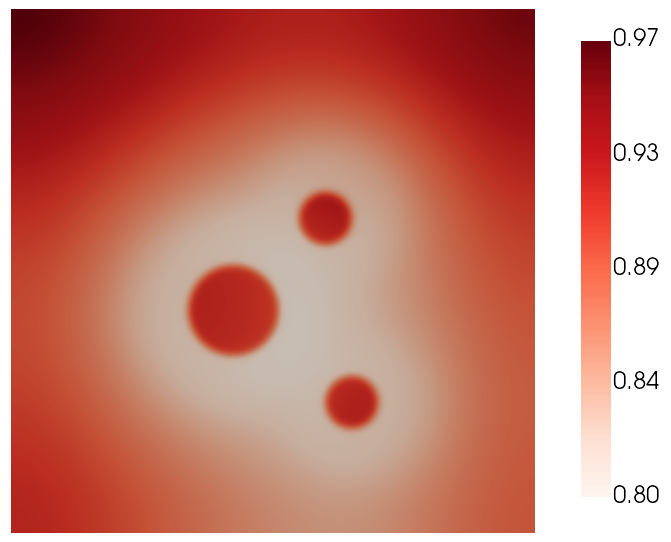
\includegraphics[scale=0.145]{img/three_tumors/test_DG_P0-125_chi-10_dt-5e-6_nx-200_symmetric/tumor_DG-UPW_Pi1_n_i-3000_cropped.png}} &
			\raisebox{-0.47\height}{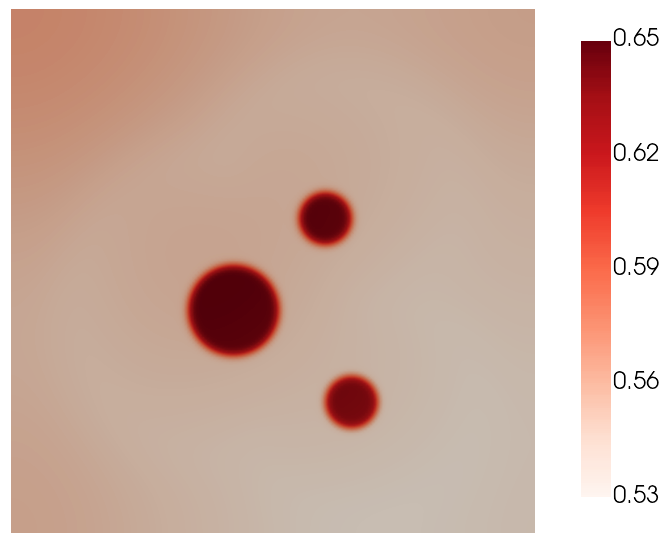
\includegraphics[scale=0.145]{img/three_tumors/test_DG_P0-125_chi-10_dt-5e-6_nx-200_symmetric/tumor_DG-UPW_Pi1_n_i-8000_cropped.png}} \\
			\rotatebox[origin=c]{90}{\textbf{FE}} &
			\raisebox{-0.47\height}{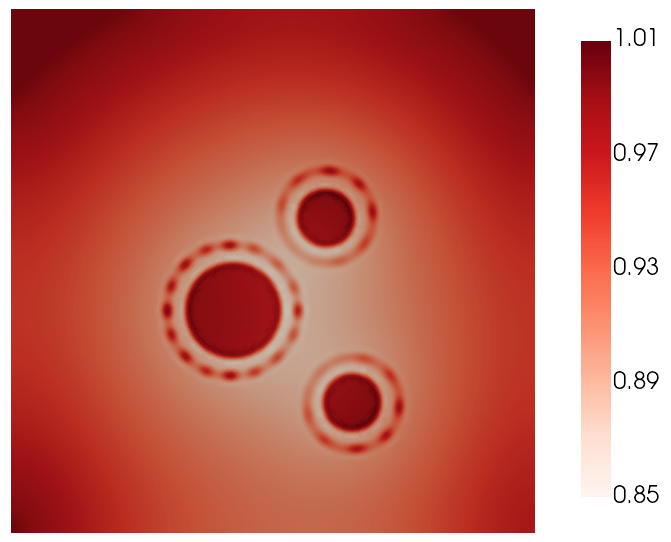
\includegraphics[scale=0.145]{img/three_tumors/test_FEM_P0-125_chi-10_dt-5e-6_nx-200_symmetric/tumor_FEM_n_i-1500_cropped.png}} &
			\raisebox{-0.47\height}{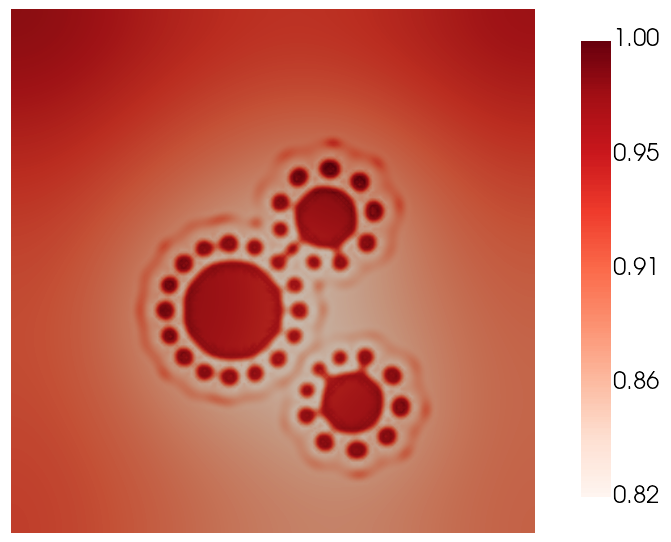
\includegraphics[scale=0.145]{img/three_tumors/test_FEM_P0-125_chi-10_dt-5e-6_nx-200_symmetric/tumor_FEM_n_i-3000_cropped.png}} &
			\raisebox{-0.47\height}{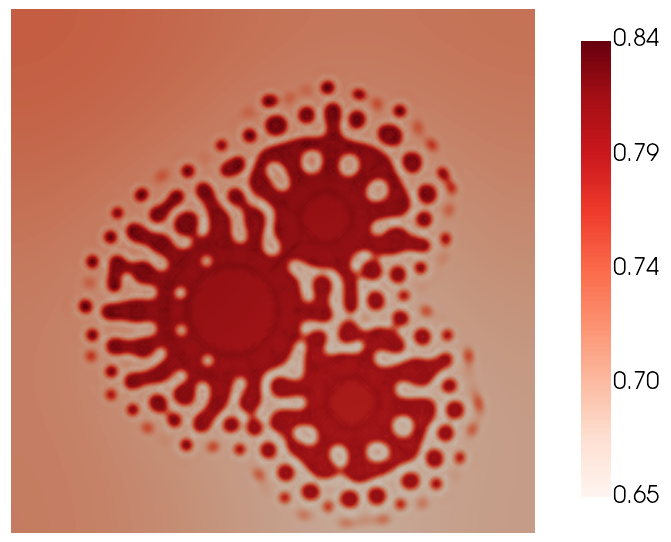
\includegraphics[scale=0.145]{img/three_tumors/test_FEM_P0-125_chi-10_dt-5e-6_nx-200_symmetric/tumor_FEM_n_i-8000_cropped.png}}
		\end{tabular}
		\caption{Nutrients.}
		\label{fig:test-1_2}
	\end{figure}
\end{frame}
\begin{frame}{Three tumors aggregation ($\chi_0=0$, $\Delta t=10^{-5}$)}
	\begin{figure}
		\centering
		\begin{tabular}{cc}
			\hspace*{1cm}$\boldsymbol{u}$ & \hspace*{0.5cm}$\boldsymbol{n}$\\
			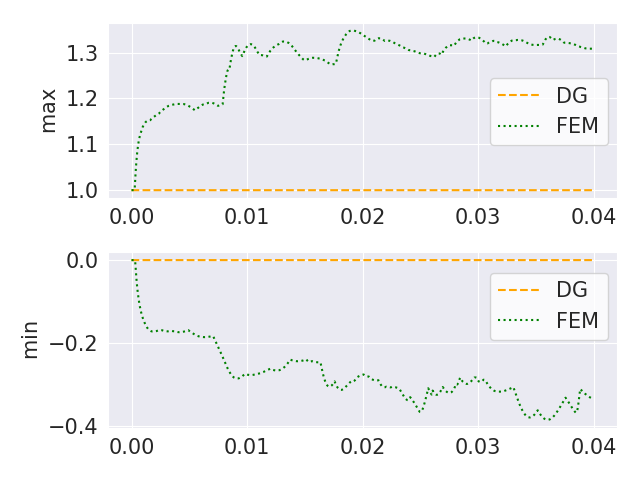
\includegraphics[scale=0.33]{img/three_tumors/tumor_min-max_u_chi-10.png} &
			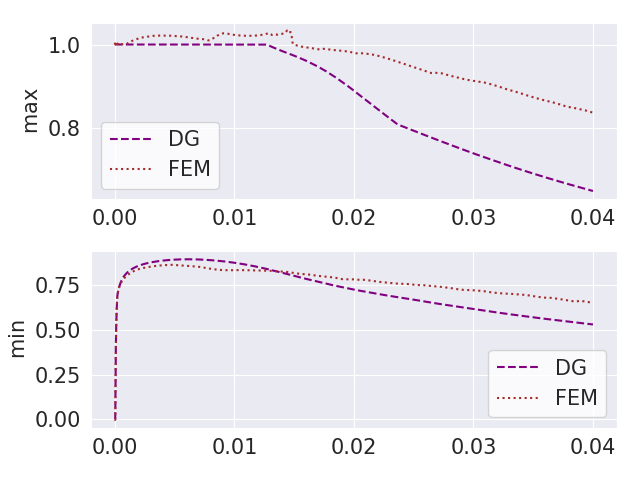
\includegraphics[scale=0.33]{img/three_tumors/tumor_min-max_n_chi-10.png}
		\end{tabular}
		\caption{Pointwise bounds.}
	\end{figure}
\end{frame}
\begin{frame}{Three tumors aggregation ($\chi_0=0$, $\Delta t=10^{-5}$)}
	\begin{figure}
		\centering
		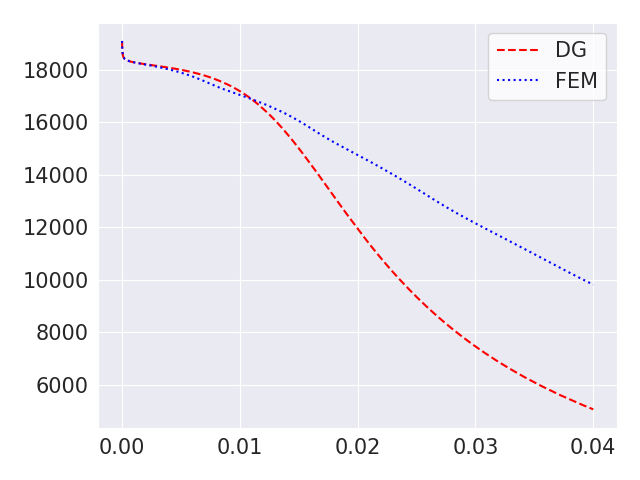
\includegraphics[scale=0.45]{img/three_tumors/tumor_energy_chi-10.png}
		\caption{Energy.}
	\end{figure}
\end{frame}

\subsection{Irregular tumor growth}

\begin{frame}{Irregular tumor growth {\footnotesize (more tests in \cite{acosta2023structure})}}
	\footnotesize
	\begin{figure}
		\centering
		\begin{tabular}{cc}
			\hspace*{-1.1cm}$\boldsymbol{u_0}$ & \hspace*{-1.1cm}$\boldsymbol{n_0}$\\
			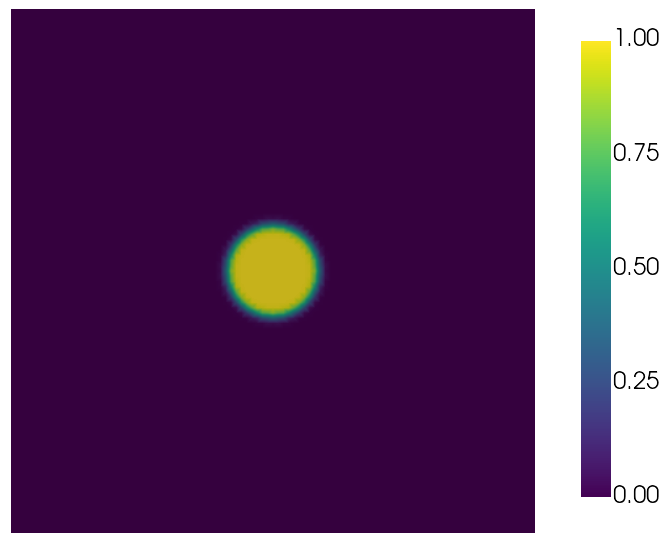
\includegraphics[scale=0.2]{img/irregular_shape/initial_cond/tumor_DG-UPW_Pi1_u_i-0_cropped.png} &
			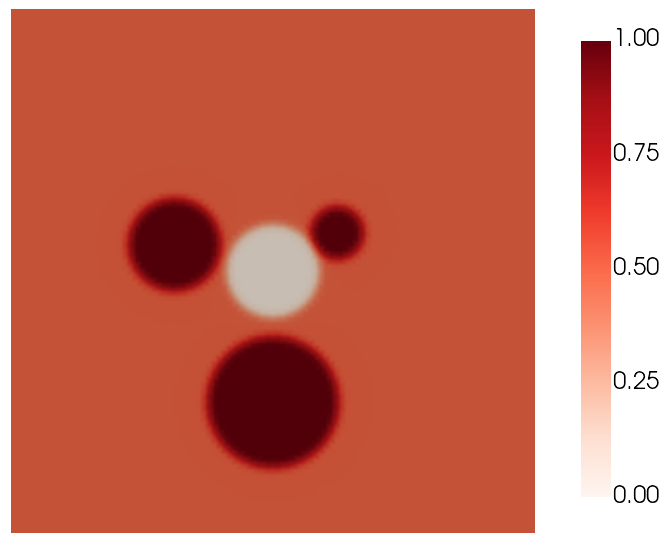
\includegraphics[scale=0.2]{img/irregular_shape/initial_cond/tumor_DG-UPW_Pi1_n_i-0_cropped.png}
		\end{tabular}
	\end{figure}

	Symmetric mobility and proliferation functions:
	$$
	M(v)=h_{1,1}(v),\quad P(u,n)=h_{1,1}(u)n_\oplus.
	$$
	Nonsymmetric mobility and proliferation functions:
	$$
	M(v)=h_{5,1}(v),\quad P(u,n)=h_{1,3}(u) n_\oplus.
	$$

	Parameters: $C_u=2.8$, $C_n=2.8\cdot 10^{-4}$, $h\approx 0.28$, $P_0=0.5$, $\chi_0=0.1$, $\Delta t=0.1$.
\end{frame}
\begin{frame}{Irregular tumor growth {\footnotesize (more tests in \cite{acosta2023structure})}}
	\scriptsize
	\begin{figure}
		\centering
		\hspace*{-0.6cm}
		\begin{tabular}{ccccc}
			& \hspace*{-1cm}$t=10.0$ & \hspace*{-1cm}$t=20.0$ & \hspace*{-1cm}$t=50.0$ \\
			\rotatebox[origin=c]{90}{\textbf{Symmetric}} &
			\raisebox{-0.47\height}{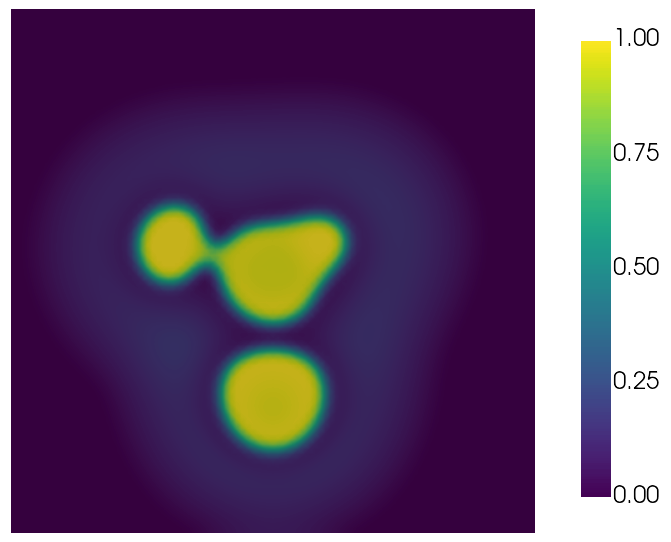
\includegraphics[scale=0.145]{img/irregular_shape/reference_test_symmetric/tumor_DG-UPW_Pi1_u_i-100_cropped.png}} &
			\raisebox{-0.47\height}{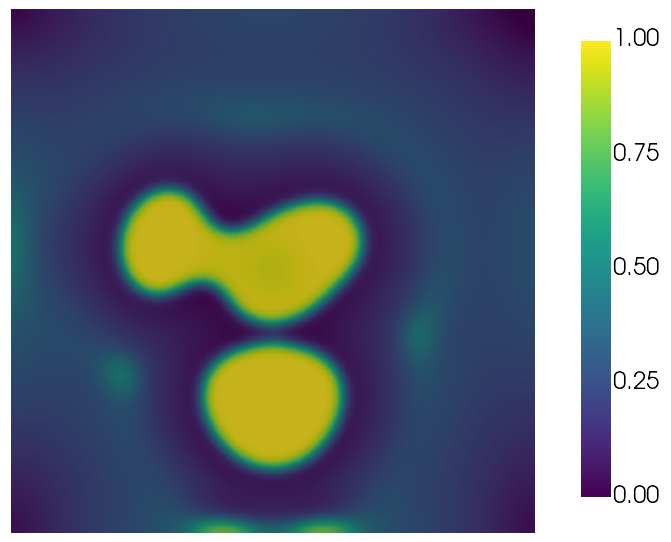
\includegraphics[scale=0.145]{img/irregular_shape/reference_test_symmetric/tumor_DG-UPW_Pi1_u_i-200_cropped.png}} &
			\raisebox{-0.47\height}{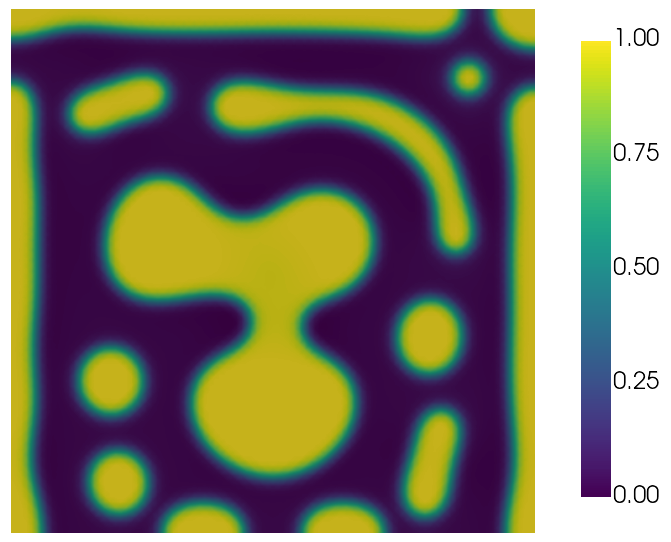
\includegraphics[scale=0.145]{img/irregular_shape/reference_test_symmetric/tumor_DG-UPW_Pi1_u_i-500_cropped.png}} \\
			\rotatebox[origin=c]{90}{\textbf{Non-symmetric}} &
			\raisebox{-0.47\height}{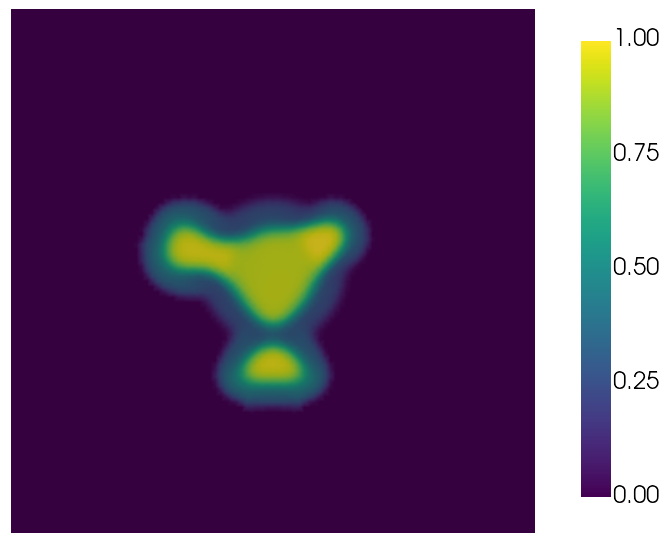
\includegraphics[scale=0.145]{img/irregular_shape/reference_test/tumor_DG-UPW_Pi1_u_i-100_cropped.png}} &
			\raisebox{-0.47\height}{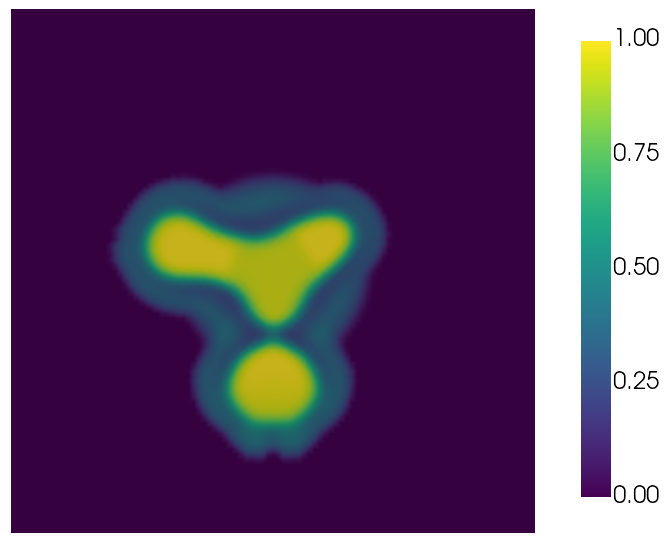
\includegraphics[scale=0.145]{img/irregular_shape/reference_test/tumor_DG-UPW_Pi1_u_i-200_cropped.png}} &
			\raisebox{-0.47\height}{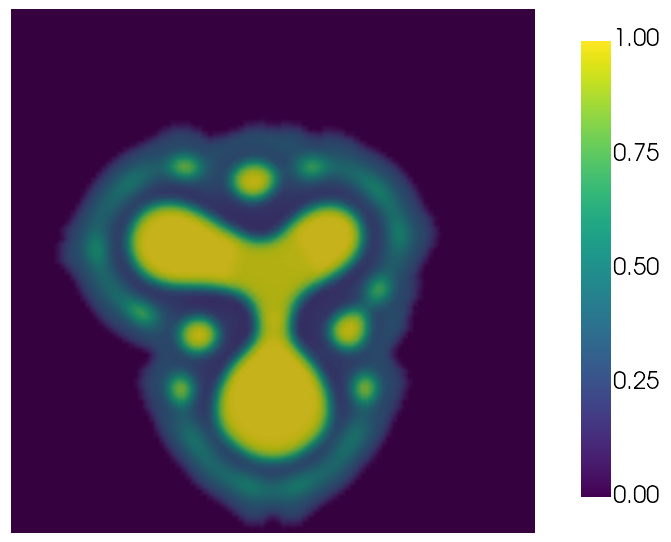
\includegraphics[scale=0.145]{img/irregular_shape/reference_test/tumor_DG-UPW_Pi1_u_i-500_cropped.png}}
		\end{tabular}
		\caption{Tumor cells.}
		\label{fig:test-2_reference}
	\end{figure}
\end{frame}
\begin{frame}{Irregular tumor growth {\footnotesize (more tests in \cite{acosta2023structure})}}
	\scriptsize
	\begin{figure}
		\centering
		\hspace*{-0.6cm}
		\begin{tabular}{ccccc}
			& \hspace*{-1cm}$t=10.0$ & \hspace*{-1cm}$t=20.0$ & \hspace*{-1cm}$t=50.0$ \\
			\rotatebox[origin=c]{90}{\textbf{Symmetric}} &
			\raisebox{-0.47\height}{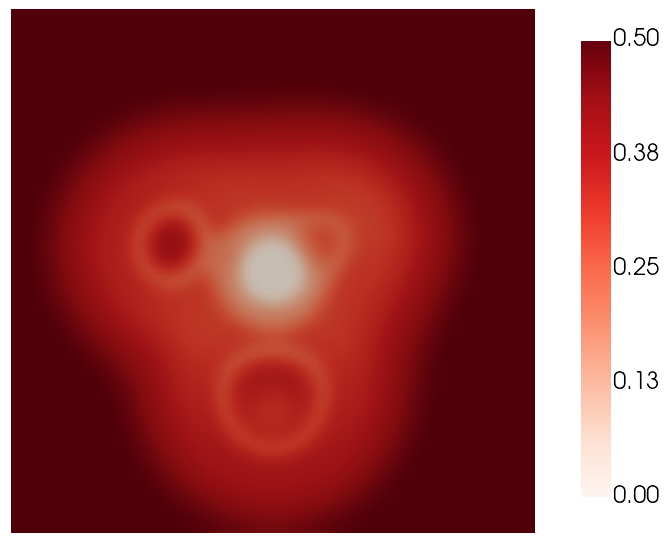
\includegraphics[scale=0.145]{img/irregular_shape/reference_test_symmetric/tumor_DG-UPW_Pi1_n_i-100_cropped.png}} &
			\raisebox{-0.47\height}{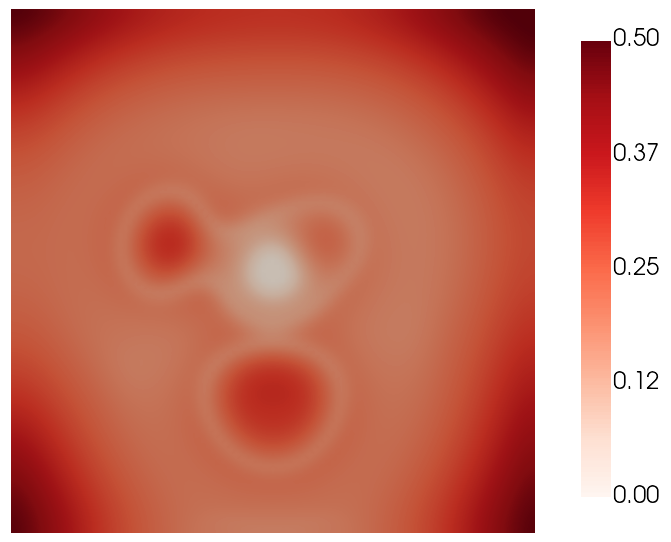
\includegraphics[scale=0.145]{img/irregular_shape/reference_test_symmetric/tumor_DG-UPW_Pi1_n_i-200_cropped.png}} &
			\raisebox{-0.47\height}{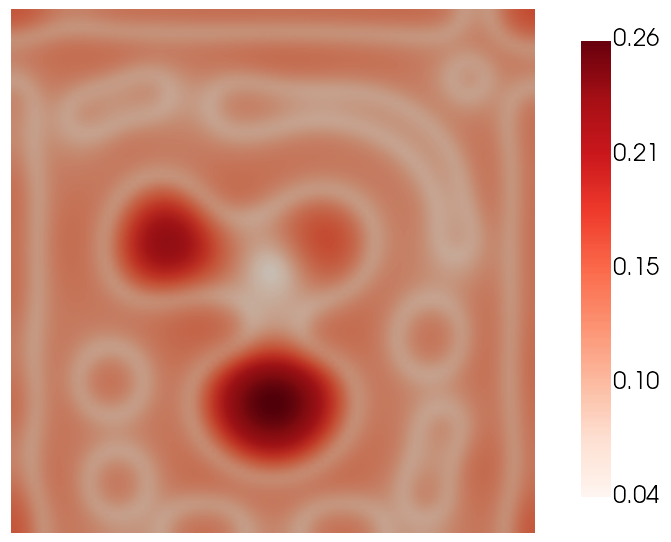
\includegraphics[scale=0.145]{img/irregular_shape/reference_test_symmetric/tumor_DG-UPW_Pi1_n_i-500_cropped.png}} \\
			\rotatebox[origin=c]{90}{\textbf{Non-symmetric}} &
			\raisebox{-0.47\height}{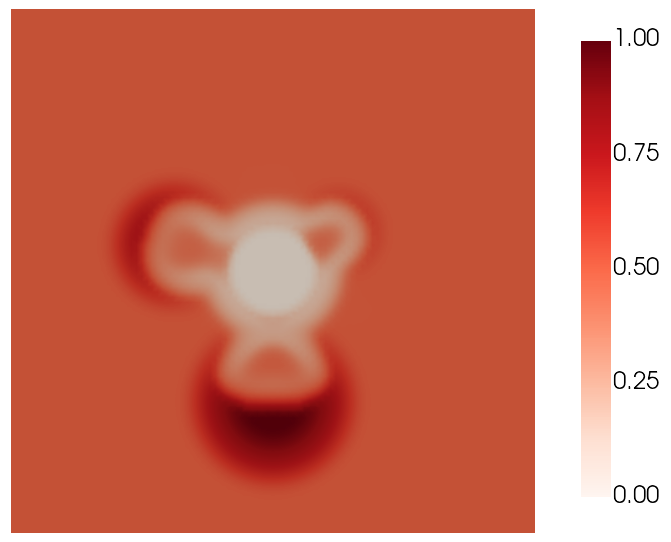
\includegraphics[scale=0.145]{img/irregular_shape/reference_test/tumor_DG-UPW_Pi1_n_i-100_cropped.png}} &
			\raisebox{-0.47\height}{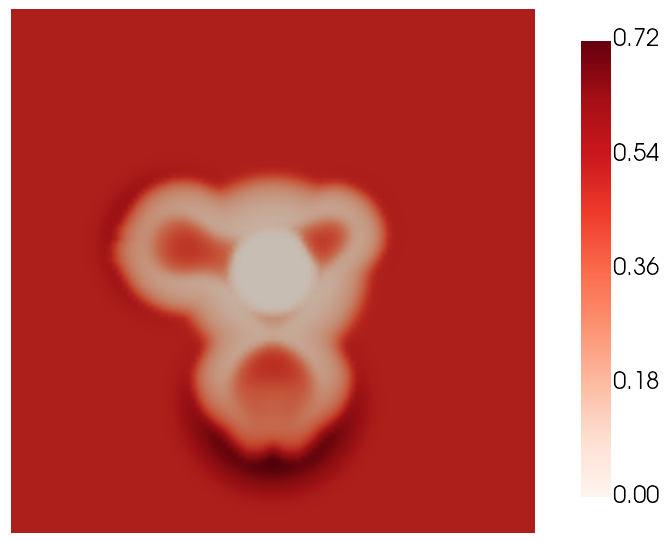
\includegraphics[scale=0.145]{img/irregular_shape/reference_test/tumor_DG-UPW_Pi1_n_i-200_cropped.png}} &
			\raisebox{-0.47\height}{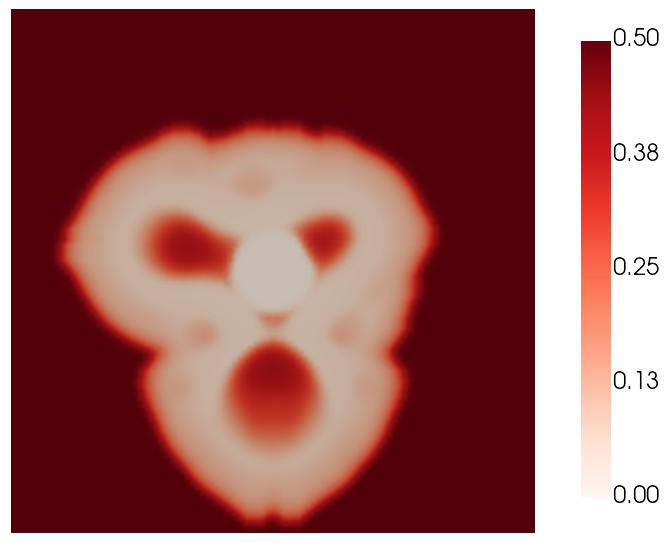
\includegraphics[scale=0.145]{img/irregular_shape/reference_test/tumor_DG-UPW_Pi1_n_i-500_cropped.png}}
		\end{tabular}
		\caption{Nutrients.}
	\end{figure}
\end{frame}

\begin{frame}{References}
	\scriptsize 
	\vspace*{-0.25cm}
	\nocite*
	\bibliographystyle{apalike}
	\bibliography{references}
\end{frame}

\begin{frame}{}
	\centering
	\vspace*{1cm}
	{\Huge
		\emph{Thanks for your attention!}}
	
	\vspace*{0.5cm}
	\emph{Happy birthday Giuseppe!}
	
	\vspace*{1cm}
	\begin{acknowledgements}
		The speaker has been supported by a \textit{Graduate Scholarship funded by the University of Tennessee at Chattanooga}; by \textit{UCA FPU contract UCA/REC14VPCT/2020, Erasmus+ KA131 and travel grants funded by Universidad de Cádiz}.
		
		The collaborators have been supported by \textit{Grant US-4931381261 (US/JUNTA/FEDER, UE)}.
	\end{acknowledgements}
\end{frame}